\chapter{Dados Pseudo-Experimentais}

\section{Resposta do sistema no tempo} \label{Resposta do sistema no tempo}

Para a construção dos dados pseudo-experimentais foram observados os seguintes casos:

Forçamento:
\begin{itemize}
	\item $F_0(t) = A_0 sin(2\pi f_0 t)$ 
	(Considere $\frac{\omega_1}{2\pi} \leq f_0 \leq \frac{\omega_2}{2\pi})$ 
	\item $F_1(t) = A_1 sin(2\pi f_1 t) + A_2 sin(2\pi f_2 t)$ 
	(Escolha 
	$\frac{0.8 \omega_1}{2\pi} \leq f_j \leq \frac{1.2 \omega_2}{2\pi}$ 
	e
	$A_2 = 2A_1$
	;
	$ j = 1, 2)$
	\item $F_2(t) = $ ruído branco
\end{itemize}

Número de amostras $N$:
\begin{itemize}
	\item $N = 1000$
	\item $N = 5000$
\end{itemize}

Valores para a relação entre sinal e ruído - \abbrev{SNR}{Signal to Noise Ratio} SNR (Signal to Noise Ratio):
\begin{itemize}
	\item $SNR = 90$
	\item $SNR = 50$
	\item $SNR = 10$
\end{itemize}

A \cref{fig:FRF_i2_o2_freq34} mostra a posição da frequência de excitação para a aplicação da força $F_0$, em que uma amplitude $A_0 = 1$ foi utilizada.

A \cref{fig:F0_1000_tempo} mostra a resposta no tempo do sistema ao aplicarmos a força $F_0$ na frequência mostrada na \cref{fig:FRF_i2_o2_freq34} para uma amostragem $N = 1000$. Podemos observar que, para $N=1000$, temos uma excitação de aproximadamente 16 segundos e ainda temos algum transiente na resposta no tempo. Também é possível observar que essa parcela apresenta mais que uma frequência de oscilação.

\begin{figure}
	\centering
	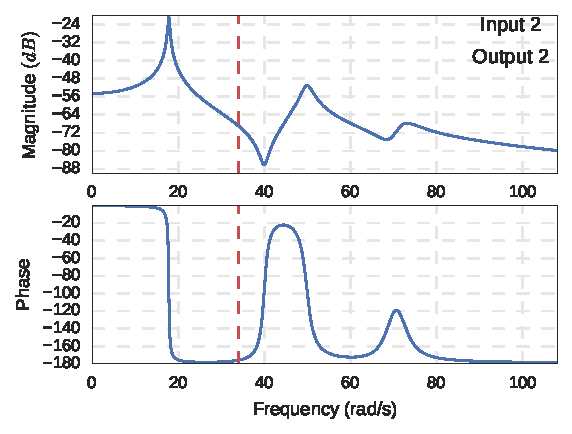
\includegraphics[scale=0.7]{FRF_i2_o2_freq34.pdf}
	\caption{Frequência de excitação para a força $F_0$.}
	\label{fig:FRF_i2_o2_freq34}
\end{figure}

\begin{figure}[h]
	\centering
	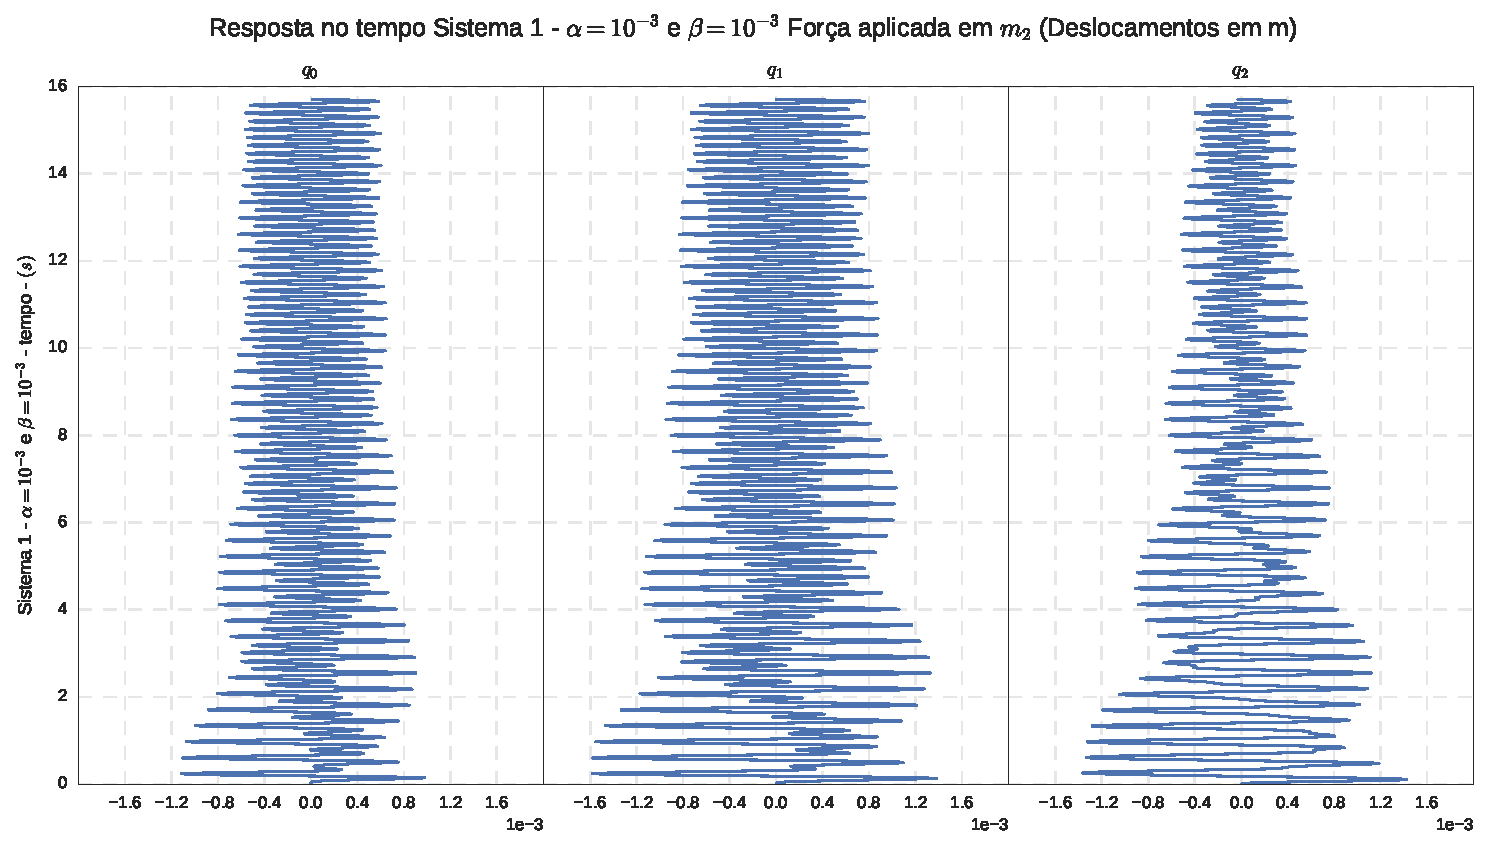
\includegraphics[scale=0.65]{F0_1000_tempo.pdf}
	\caption{Resposta no tempo para a força $F_0$ com $N=1000$.}
	\label{fig:F0_1000_tempo}
\end{figure}

A \cref{fig:F0_5000_tempo} mostra a resposta no tempo para $N=5000$. Neste caso, o tempo vai até aproximadamente 80 segundos e podemos observar que a parcela transiente é praticamente inexistente após os 20 segundos de excitação. Após esse tempo, é esperado que o sistema oscile apenas na frequência de excitação.

\begin{figure}
	\centering
	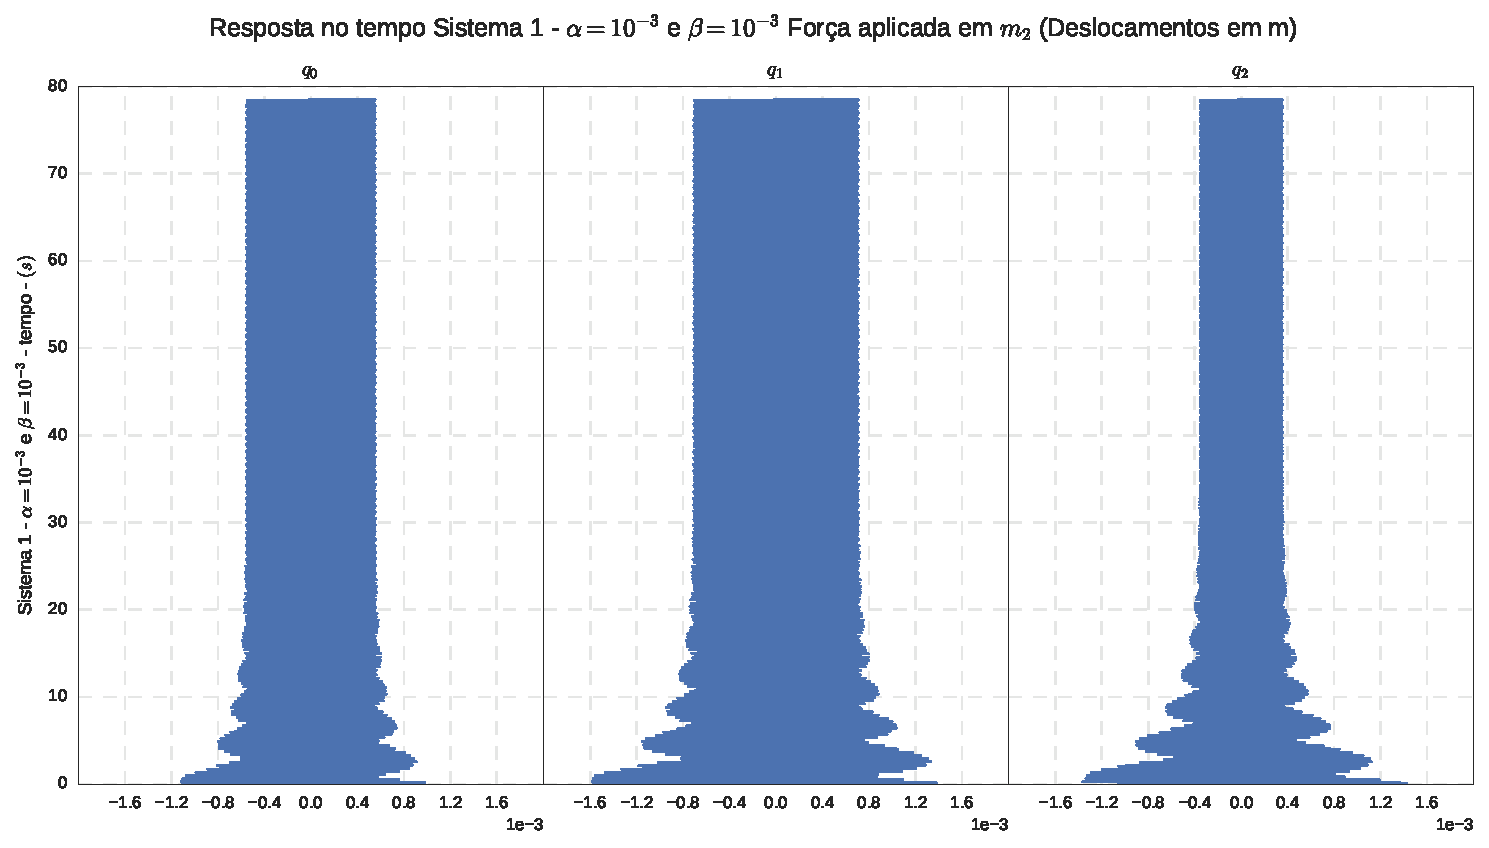
\includegraphics[scale=0.65]{F0_5000_tempo.pdf}
	\caption{Resposta no tempo para a força $F_0$ com $N=5000$.}
	\label{fig:F0_5000_tempo}
\end{figure}

Para a força $F_1$, a \cref{fig:FRF_i2_o2_freq_1_2} mostra as frequências de excitação que foram aplicadas na massa $m_2$. Podemos notar que, nesse caso, as forças aplicadas estão próximas as frequências naturais do sistema.

\begin{figure}
	\centering
	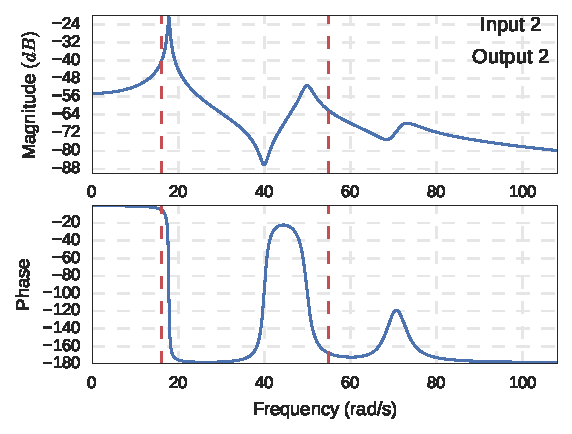
\includegraphics[scale=1]{FRF_i2_o2_freq_1_2.pdf}
	\caption{Frequência de excitação para a força $F_1$.}
	\label{fig:FRF_i2_o2_freq_1_2}
\end{figure}

A \cref{fig:F1_5000_tempo} mostra a resposta no tempo para $F_1$ com $ A_1 = 1 $, $ A_2 = 2  $ e $ N=5000 $. Como esperado, notamos um aumento na amplitude de \SI{1e-3}{\m} para \SI{1e-2}{\m} quando comparado à força $ F_0 $.

\begin{figure}
	\centering
	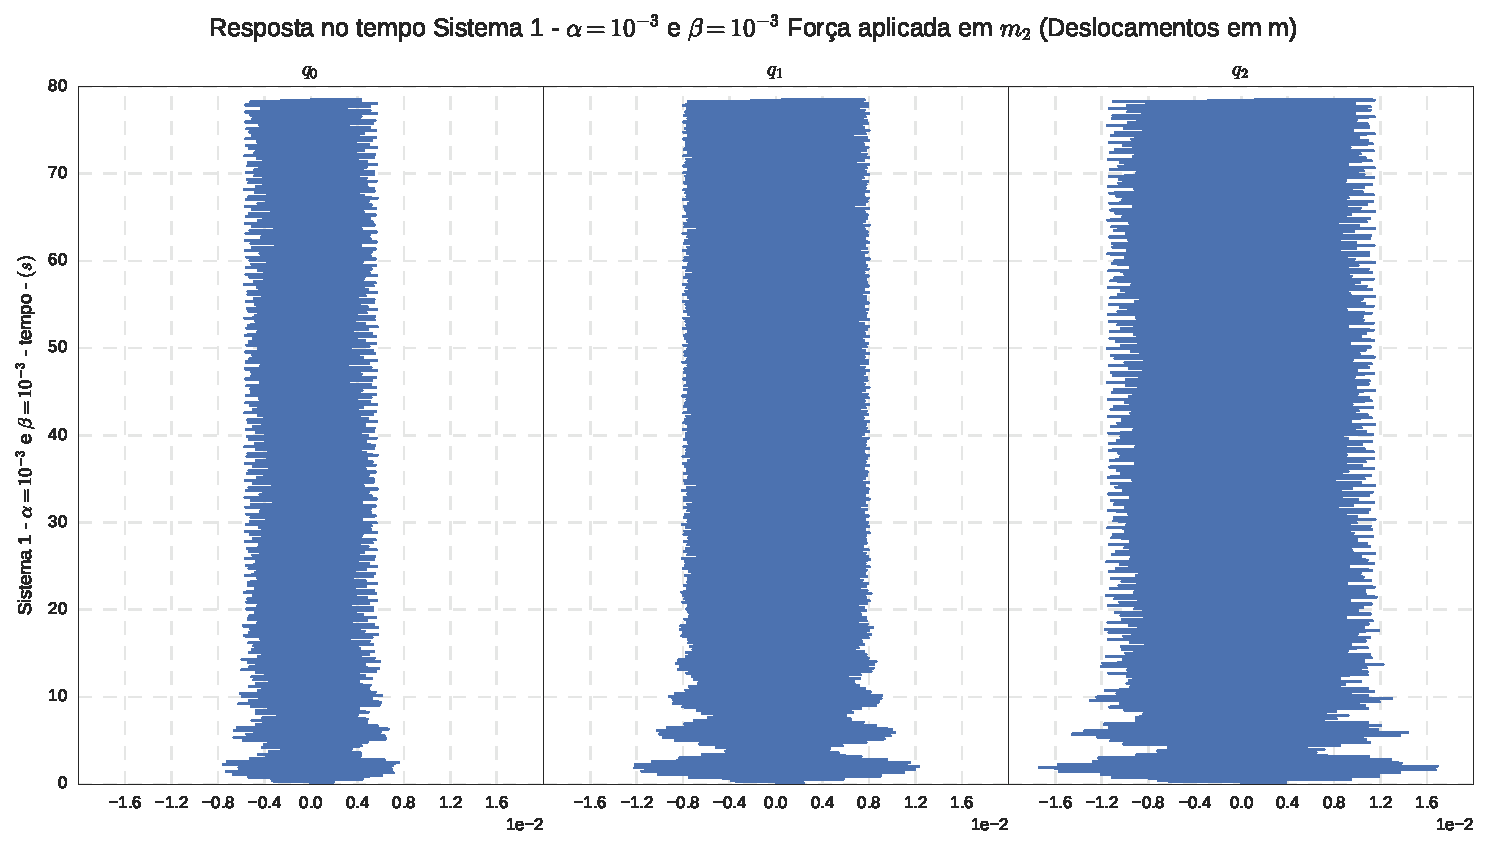
\includegraphics[scale=0.55]{F1_5000_tempo.pdf}
	\caption{Resposta no tempo para a força $F_1$ com $N=5000$.}
	\label{fig:F1_5000_tempo}
\end{figure}

O último caso de forçamento é mostrado na \cref{fig:F2_5000_tempo} onde um ruído branco com variância 1 é aplicado ao sistema.

\begin{figure}[h]
	\centering
	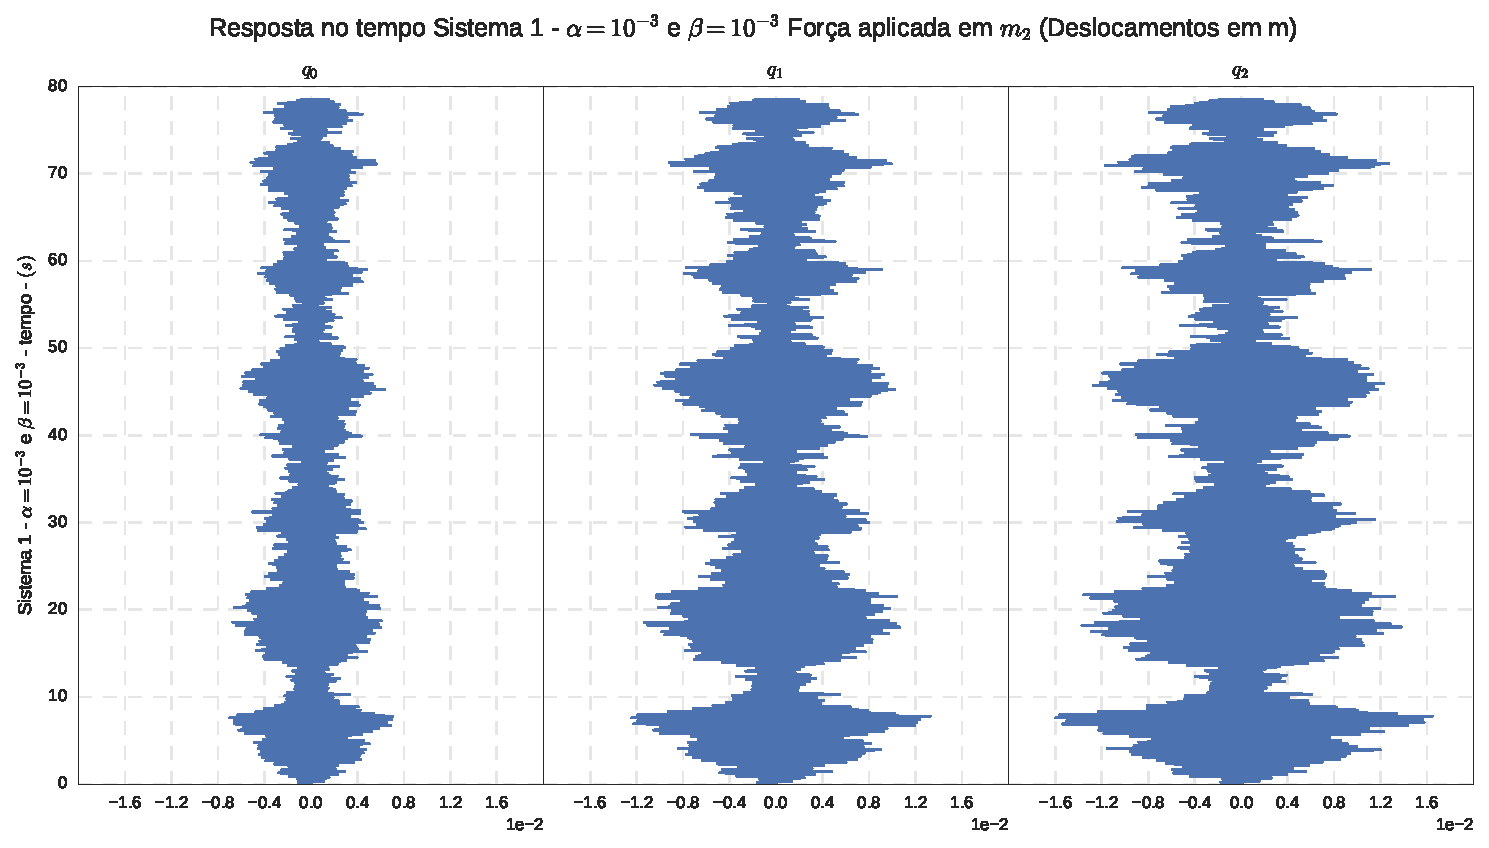
\includegraphics[scale=0.55]{F2_5000_tempo.pdf}
	\caption{Resposta no tempo para a força $F_2$ com $N=5000$.}
	\label{fig:F2_5000_tempo}
\end{figure}

\clearpage \section{Adição do ruído}

Conforme mostrado no item \ref{Resposta do sistema no tempo}, a análise será feita para três diferentes níveis de ruído ($ SNR $ = 90, 50, 10). 

Temos então que o sinal utilizado para o projeto do filtro será:

\begin{equation}
y = y^{ideal} + n
\end{equation}
onde $ n $ representa um ruído inserido no sinal.

Para calcularmos a amplitude do ruído inserido '$ n $' utilizaremos a \cref{eq:snr}.

\begin{equation} \label{eq:snr}
SNR = 20log_{10}\Bigg(\frac{A_s}{A_n}\Bigg) \rightarrow A_n = \frac{A_s}{10^{SNR/20}}
\end{equation}

Abaixo (\cref{fig:F0_noise_90} e \cref{fig:F0_noise_10}), são mostrados alguns resultados comparando o sinal puro e o sinal corrompido para um determinado nível de ruído.

\begin{figure}[h]
	\centering
	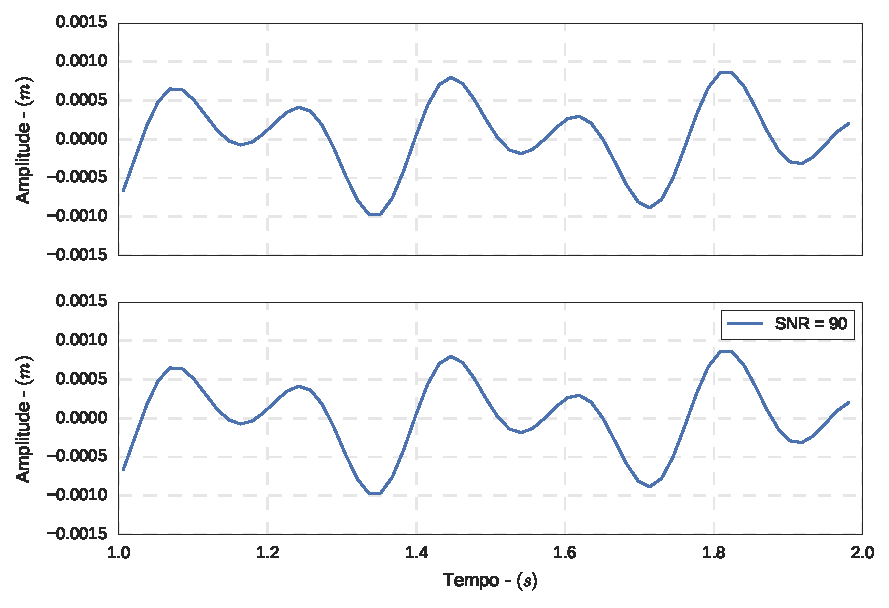
\includegraphics[scale=0.6]{F0_noise_90}
	\caption{Sinal puro e sinal corrompido para $ F_0 $ e $ SNR=90 $.}
	\label{fig:F0_noise_90}
\end{figure}

\begin{figure}
	\centering
	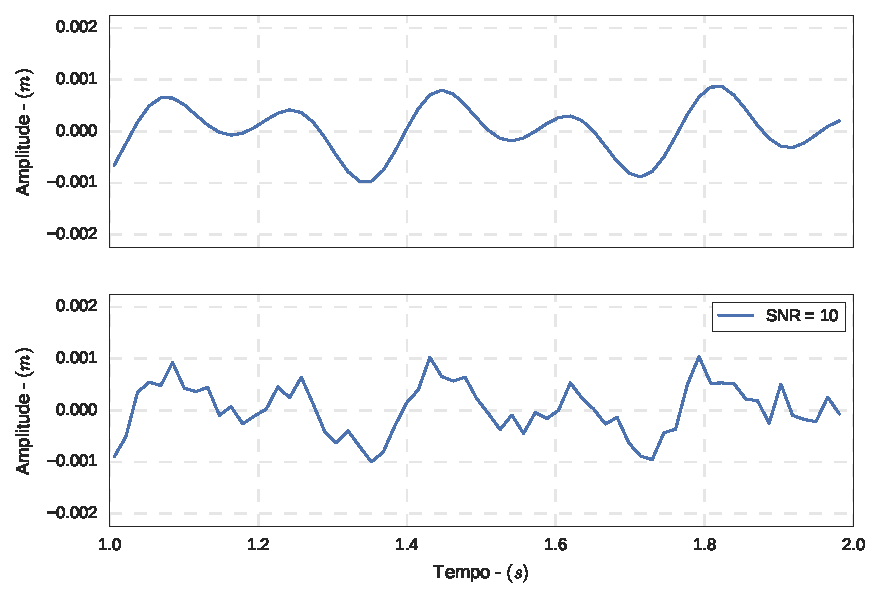
\includegraphics[scale=0.6]{F0_noise_10}
	\caption{Sinal puro e sinal corrompido para $ F_0 $ e $ SNR=10 $.}
	\label{fig:F0_noise_10}
\end{figure}
